%% uctest.tex
%% See accompanying LICENSE file for licensing, history, and copyright
%% information.

% This line is required for LPPL compliance.
\message{You are using a modified uctest.tex}
% Note that if you turn this file into a Derived Work that is not intended as a
% replacement for the original template (i.e. an actual thesis), and you do not
% imply that anyone provides support for your modified version, you may
% distribute it under any license you wish.

\documentclass[11pt]{ucscthesis}
\def\dsp{\def\baselinestretch{2.0}\large\normalsize}
\dsp

% 2010june01 sol katzman:
% package geometry should override the various margin settings from .clo and .cls
% and also eliminates issues where the default papersize is A4
\usepackage[letterpaper, left=1.5in, right=1.25in, top=1.25in, bottom=1.25in, includefoot]{geometry}
% Use PostScript fonts as required by UCSC Dissertation Preparation Guidelines
\usepackage{pslatex}
\usepackage{graphicx}
\usepackage{fullpage} % Package to use full page
\usepackage{parskip} % Package to tweak paragraph skipping
\usepackage{tikz} % Package for drawing
\usepackage{amsmath}
\usepackage{hyperref}
\usepackage{graphicx}
\usepackage{figsize}

\bibliographystyle{unsrt}



\begin{document}

% Declarations for Front Matter

\title{The Elements of Project}
\author{Weiting Zhan}
\degreeyear{2019}
\degreemonth{June}
\degree{Master of Science in Computer Engineering}
\chair{Professor Roberto Manduchi}
\committeememberone{Professor J. J. Garcia-Luna-Aceves}



\campus{Santa Cruz}

\begin{frontmatter}

\maketitle


\tableofcontents
\listoffigures

\begin{abstract}
According to the World Health Organization, it is estimated that globally approximately 1.3 billion people live with some form of vision impairment. In this project, the author developed an IOS application and an Android application, both named ISee, for blind or visually impaired users. Both applications take a picture as input, use Google Firebase MLKit to recognize the character and entities in an image, and then read the text or content of the image to users. ISee used the most advanced Optical Character Recognition and Image Labeling Application programming interface to help blind or visually impaired users get some information about the environment. In order to evaluate the performance of the blur text recognition Algorithm developed by Siyang Qin with ML kit, the author computes the false positive rate and truth positive rate of each of them.

\end{abstract}




\end{frontmatter}



\chapter{Introduction}
 7,675,600 people in the United States reported having a visual disability in 2016, according to the National Federation of the Blind\cite{USBlindStatistics}. Globally, it is estimated that approximately 1.3 billion people live with some form of vision impairment according to World Health Organization\cite{WHOlindStatistics}.

\section{What is Optical Character Recognition and Image Labeling?}
Computer stores an image as a stream of raw numbers from a camera sensor, typically an array of color intensities of BGR (Blue, green, Red), as shown in Fig \ref{Image}. 


\begin{figure}
    \centering
    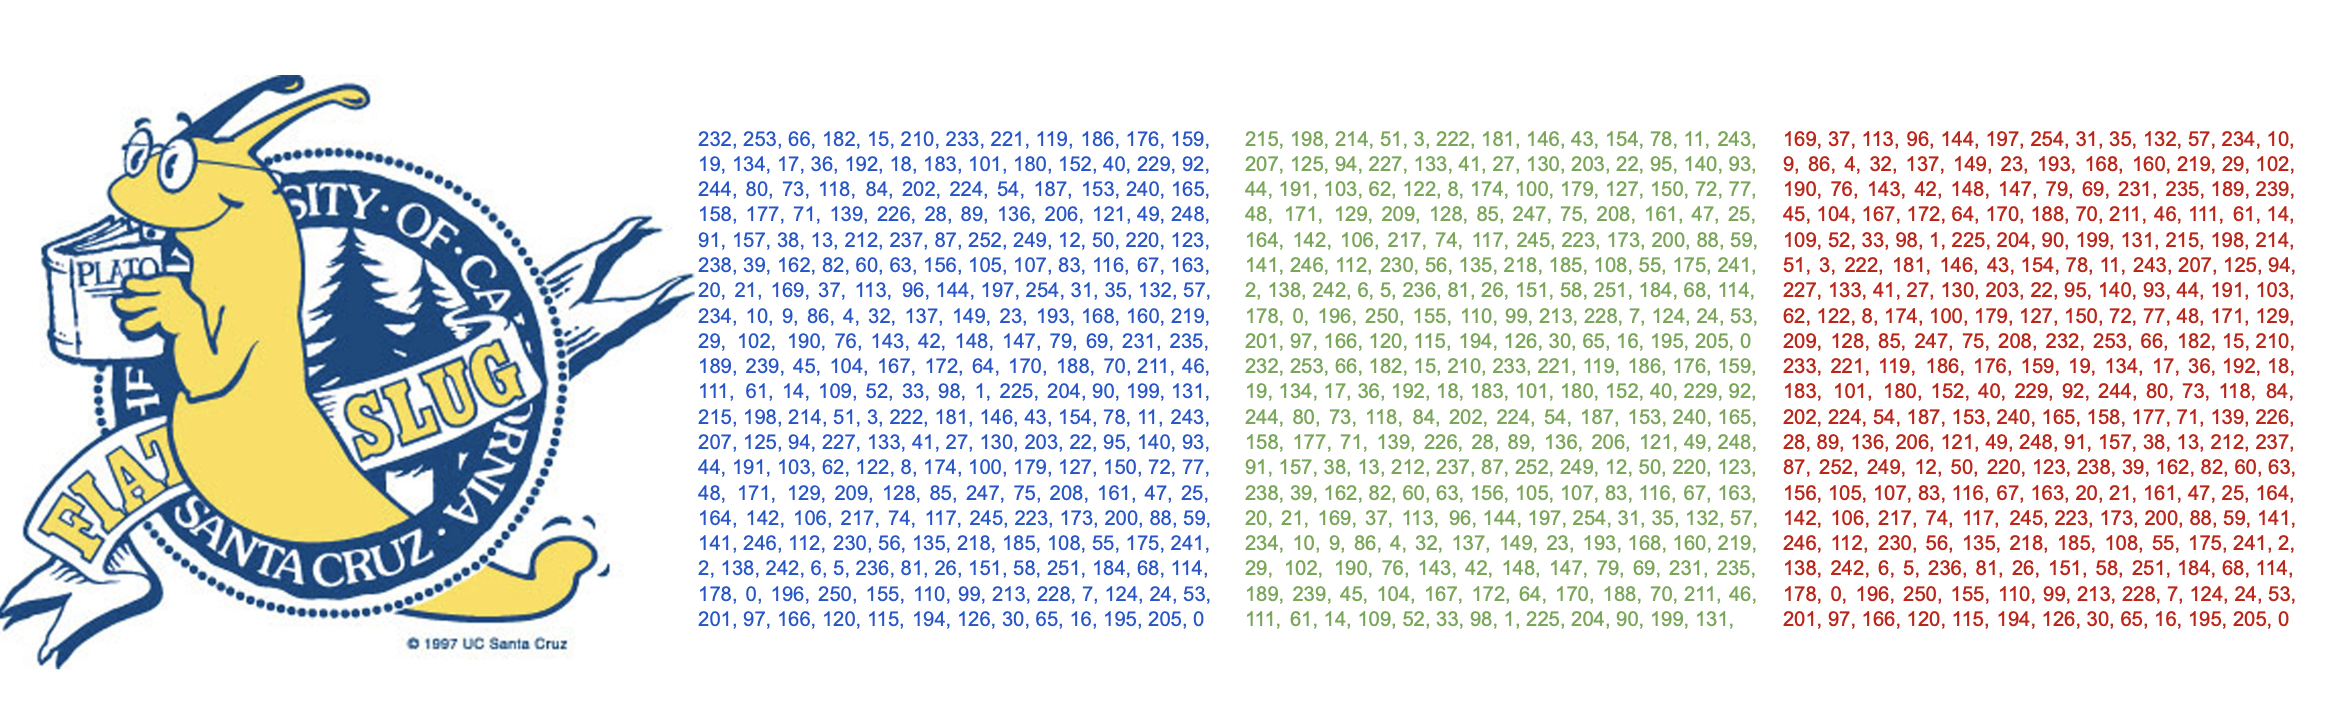
\includegraphics[width =0.8\linewidth]{Fig/image.png}
    \caption{Image stored in computer}
    \label{Image}
\end{figure}


Optical Character Recognition (OCR) transforms images (an array of numbers) into machine-processed text, which is usually encoded using a representing scheme. So we can use a statistic classification method \cite{kotsiantis2006machine}\cite{kotsiantis2007supervised}\cite{nickel2015review} to separate one group of numbers (for example, all the images of A in the data set) from another group of numbers (all the images of B in the data set).  


Google's\cite{GoogleDocumentTextTutorial} OCR system, is periodically tested on 232 languages in 30 distinct scripts, achieving state of the art accuracy for most of image types ranging from scanned documents to casual photos.

\begin{figure}
    \centering
    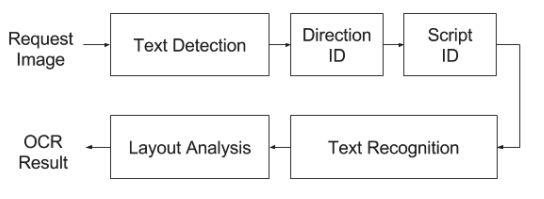
\includegraphics[width =0.8\linewidth]{Fig/googleOCRpipeline.png}
    \caption{Google Cloud Vision API Architecture \cite{GoogleDocumentTextTutorial}}
    \label{Google Document Text Tutorial}
\end{figure}



Label detection\cite{MLImageLable} predicts the most appropriate labels that describe an image, as shown in Fig \ref{MLkitImage labeling}.


\section{Optical Character Recognition with Firebase MLkit}
Building a Convolutional Neural Network from scratch and collecting enough data \cite{GoogleDatasets} to train the model is a time-consuming and expensive undertaking. 

Google Firebase ML kit \cite{GoogleMLkit} has APIs for common mobile use cases: recognizing text, detecting faces, scanning barcodes, labeling images, and recognizing landmarks. Other options are IBM Watson Visual Recognition \cite{IBMclassifier}, part of the Watson Developer Cloud and Clarif.ai \cite{clarif}. Here, we use Google Firebase MLkit to build an application for Google's large dataset and computation power.

\begin{figure}
    \centering
    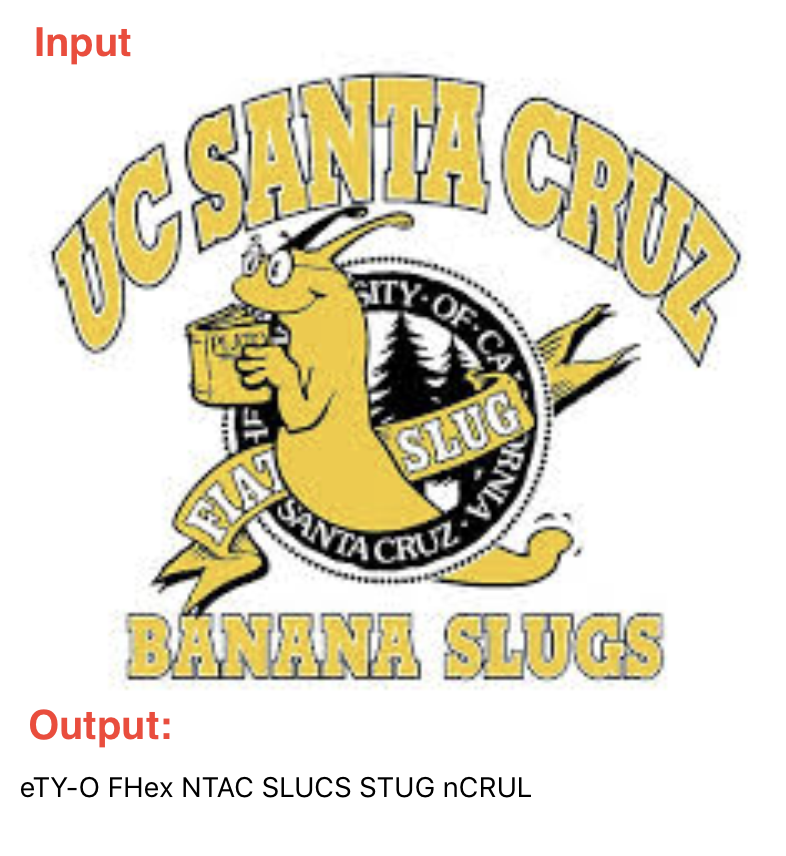
\includegraphics[width =0.4\linewidth]{Fig/OCRdemo.png}
    \caption{Google Firebase MLkit text recognition}
    \label{MLkitOCR}
\end{figure}

\section{Image labeling with Firebase MLkit}
Firebase Image labeling \cite{MLImageLable} gives insight into the content of images. 
\begin{figure}
    \centering
    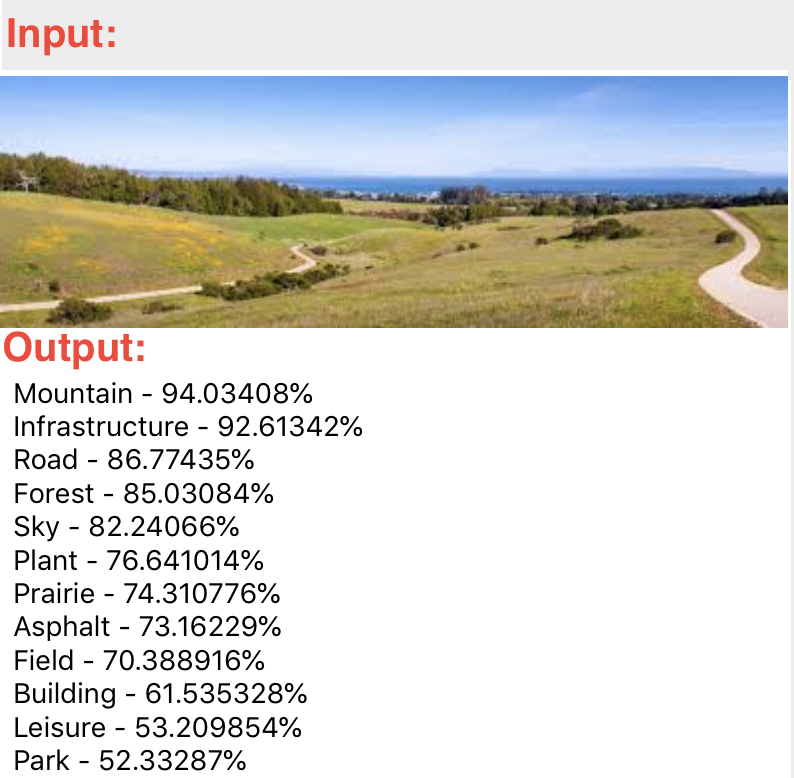
\includegraphics[width =0.5\linewidth]{Fig/Imagelabelingdemo.png}
    \caption{Google Firebase MLkit Image labeling demo}
    \label{MLkitImage labeling}
\end{figure}
The Image labeling on-device offers 400+ labels that cover the most commonly-found concepts in photos, and the cloud offers 10,0000+ labels in many categories, as shown in Fig \ref{Firebase MLkitImage labeling}
\begin{figure}
    \centering
    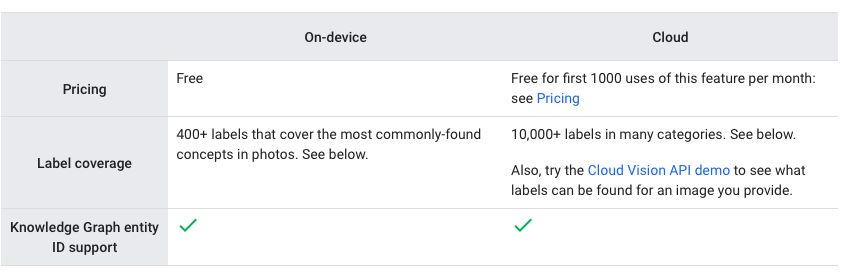
\includegraphics[width =0.5\linewidth]{Fig/FirebaseImageLabeling.png}
    \caption{Google Firebase MLkit Image labeling API\cite{MLImageLable}}
    \label{Firebase MLkitImage labeling}
\end{figure}

\section{Text to Speech API}
With the release of iOS 7, Apple introduced a text to speech API, AVSpeechSynthesizer class\cite{AVSpeechSynthesizer}, that allows developers to add text to speech functionality to an application quickly and easily.

Android Text to speech (TTS)\cite{TTSandroid} allows developers to add text to speech, and Android TTS was available from version 1.6.

\section{Blur Text recognition Algorithm}
The Blur Text recognition algorithm \cite{qin2016fast} is developed by Siyang Qin. In the project, the author compared the result of MLkit OCR with work from The Blur Text recognition algorithm \cite{qin2016fast}.




\chapter{Related Work}
\section{Apple Store}
\begin{figure}
    \centering
    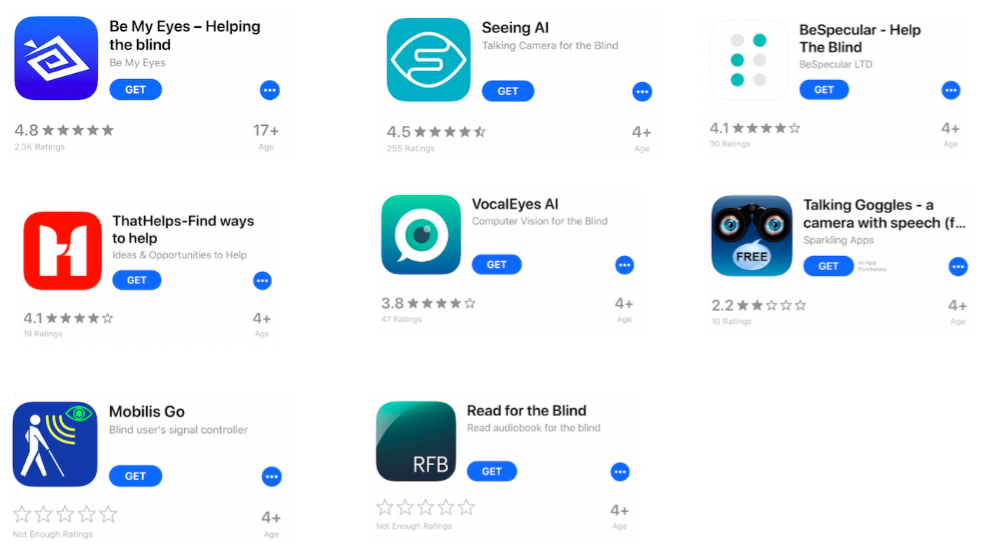
\includegraphics[width =0.8\linewidth]{Fig/AppleBlind.png}
    \caption{Application for blind user in Apple Store}
    \label{Application for blind user in Google Play Store}
\end{figure}

In the Apple store,  \textbf{\textit{Talking Googles - a camera with speech}} can recognize images and say what it finds. It can recognize almost any logo, landmark, book, product, artwork, text. It has a video model that continuously checks the video stream for identities and says them. \textbf{\textit{ThatHelps-Find ways to help}} serves to connect the volunteer with a blind user. \textbf{\textit{Be My Eyes - Helping the blind}} is also a social network connects volunteer to blind user.\textbf{\textit{Seeing AI}}, developed by Microsoft, uses the phone's camera to read what it sees automatically. It can read short text,document,product,person,currency,scene,color,handwriting to user. \textbf{\textit{BlindWays:bus stop navigation}}. help guide blind user to within a cane's distance of an outdoor bus stop sign using permanent landmark clues contributed by volunteers.\textbf{\textit{BeSpecular}}, volunteer help blind by listening to the question sent by blind, or looking at the pictures, and reply with a friendly voice note or text message.\textbf{\textit{Read for the Blind}} create audio books for the blind, by reading books or short articles from magazines, newspapers or any interesting websites.\textbf{\textit{VocalEyes AI, computer vision for the blind}}, created at MIT, identify objects, food, animals,currency and products, as well as read text, detect faces, recognize emotions and describe environments using AI. 
 \textbf{\textit{Mobilis Go}} is designed for the blind or visually impaired user. The application uses Bluetooth LE protocol to activate beacons. Activates sound beacons located on objects (like doorways, traffic lights.) Beacons emit a sound to help the user to navigate.



\section{Google Play Store}
\begin{figure}
    \centering
    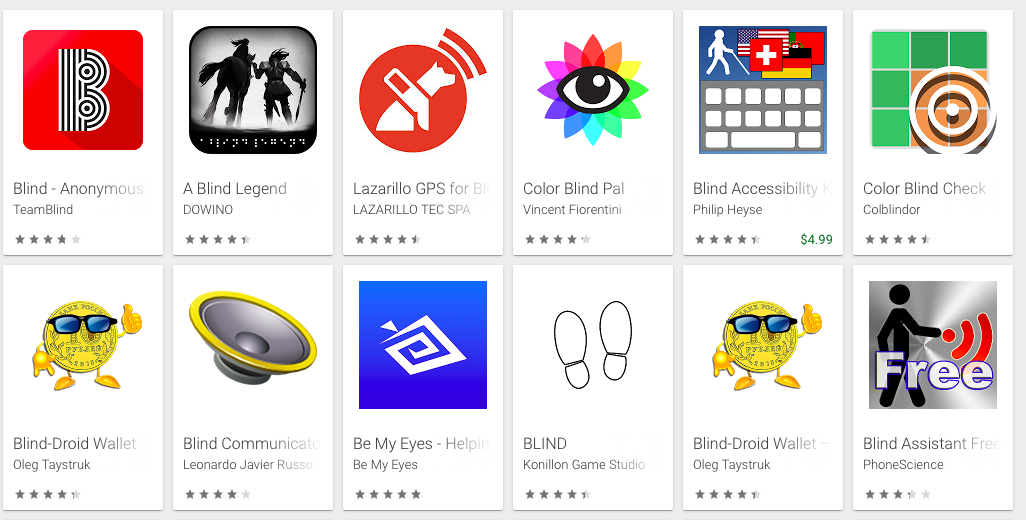
\includegraphics[width =0.8\linewidth]{Fig/GooglePlayStore.png}
    \caption{Application for blind user in Google Play Store}
    \label{Application for blind user in Google Play Store}
\end{figure}
In the Google Play store, there are 3 types application for blind user: First, connect a blind user with volunteers.\textbf{\textit{Be My Eyes -Helping the blind}}, enables blind to receive live assistance from sighted volunteers. \textbf{\textit{BeSpecular-Help the Blind}}, connect volunteers to help the blind user to identify objects, situations or images. Second, navigation application.\textbf{\textit{Lazarillo GPS}} for Blind use audio messages to tell the visually impaired user about nearby places, the street walking on. \textbf{\textit{Blind Assistant Free}}  turns the phone into a sonar employing a speaker to emit the sound pulses and a microphone to record the return echoes to detect the presence of nearby obstacles and estimate the distance. \textbf{\textit{GetThereGPS nav}} for the blind, does not display a map, but tells where is the user and how to get to the destination.
\textbf{\textit{Blind Explorer}} is a senatorial guidance system that integrated 3D sounds and satellite navigation technologies to navigate. Third, identify entity for blind user.\textbf{\textit{VIP Code Reader}}, can detect any QR code or barcode that is present in the camera's field of vision. \textbf{\textit{}Blind-Droid Wallet} is an offline paper money recognition.\textbf{\textit{Blind Communicator}} has a voice guide that tells the user everything that it's happening in the device. \textbf{\textit{NowYouSee|A colorfull world for the color blind}}, created s precisely for the type of color blindness.


In conclusion, there are only 3 applications  \textbf{\textit{Seeing AI}},\textbf{\textit{Talking Googles - a camera with speech}} and \textbf{\textit{VocalEyes AI, computer vision for the blind}}, in Apple Store and Google Play Store that designed to describe the environments or to surround to them just by taking a picture of the environments. The API they used is unknown. This project offers more options for a blind user to choose from.


\chapter{Experiment and Result}

Since the application is built on Google Firebase MLkit, the accuracy of the ISee depends on the Google Firebase MLkit, which based on the largest dataset, most advanced algorithms and sufficient computing power.

\section{ISee on IOS device}
\subsection{Optical Character Recognition}

In order to test ISee's optical character recognition feature on IOS device, the author uses 6 indoor images and 6 outdoor images as input, and the output is shown in Fig \ref{TextindoorIOS} and Fig \ref{TextoutdoorIOS}.

\begin{figure}
\centering
\SetFigLayout{3}{2}
  \subfigure[Desk]{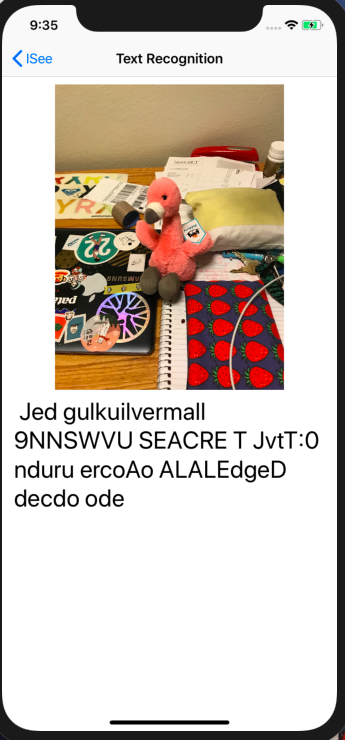
\includegraphics{Fig/FlamingoTextRecognition.png}}
  \hfill
  \subfigure[Presentation]{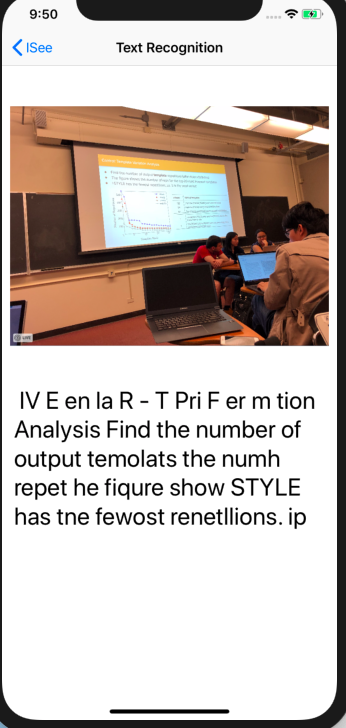
\includegraphics{Fig/ClassTextRecognition.png}}
  \hfill
  \subfigure[Comic]{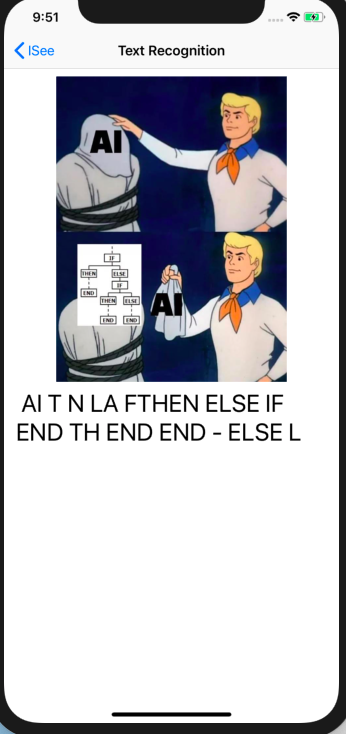
\includegraphics{Fig/AITextRecognition.png}}
  \hfill
  \subfigure[Food]{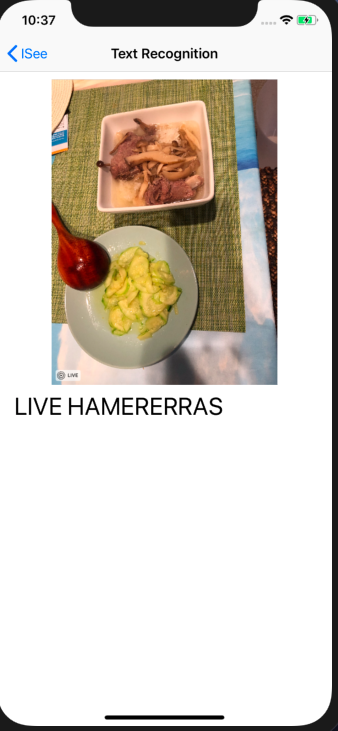
\includegraphics{Fig/foodTextRecognition.png}}
  \hfill
  \subfigure[Dancing Studio]{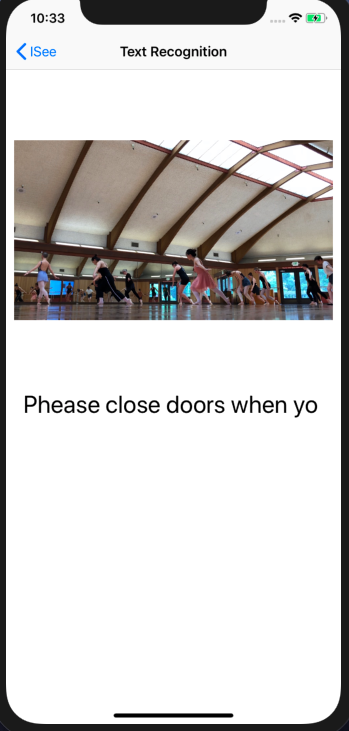
\includegraphics{Fig/BalletTextRecognition.png}}
  \hfill  
  \subfigure[Screen Shot]{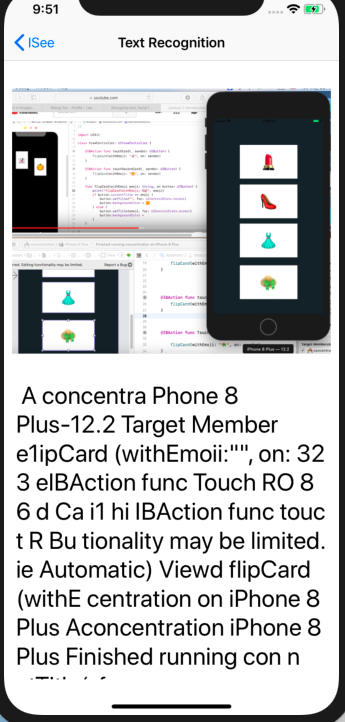
\includegraphics{Fig/ScreenshotTextRecognition.png}}
  \hfill
\caption{Indoor Image Text Recognition on IOS device}
\label{TextindoorIOS}
\end{figure}


\begin{figure}
\centering
\SetFigLayout{3}{2}
  \subfigure[Beach]{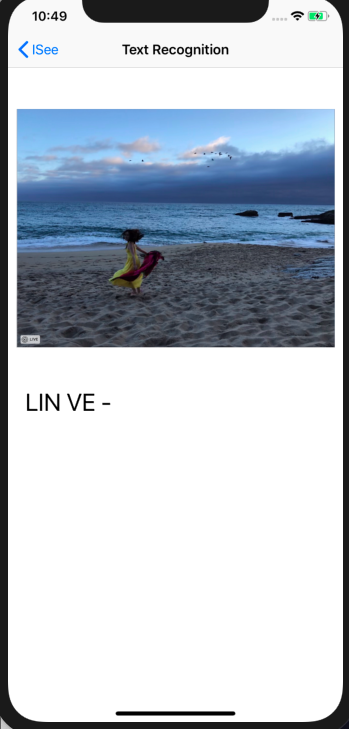
\includegraphics{Fig/BeachTextRecognition.png}}
  \hfill
  \subfigure[Road]{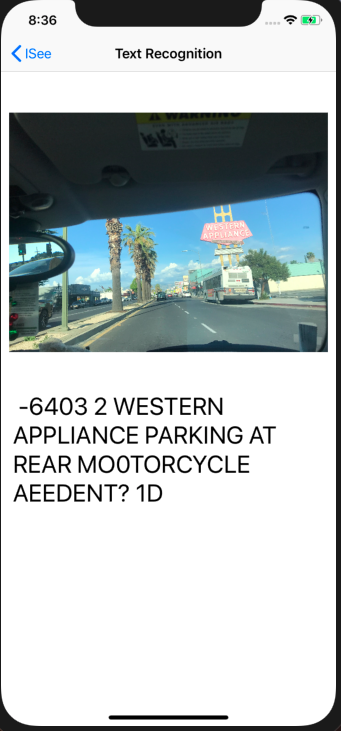
\includegraphics{Fig/carviewTextRecognition.png}}
  \hfill
  \subfigure[
signpost]{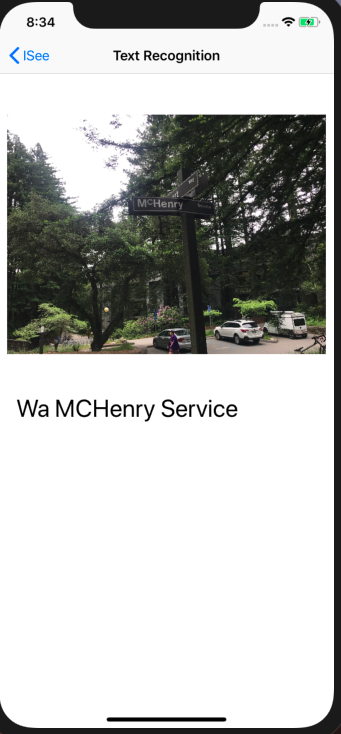
\includegraphics{Fig/signTextRecognition.png}}
  \hfill
  \subfigure[Library Sign]{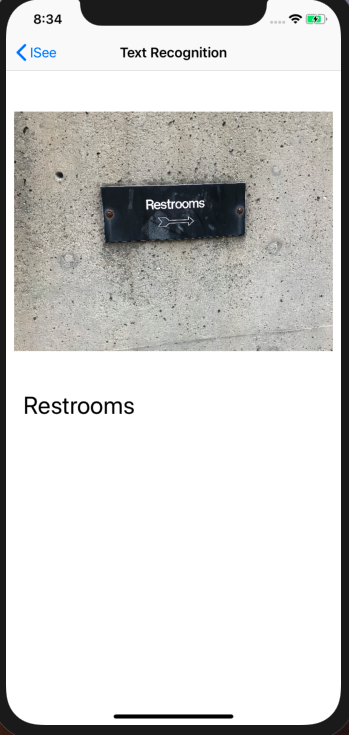
\includegraphics{Fig/RestroomsTextRecognition.png}}
  \hfill
  \subfigure[Parking lot]{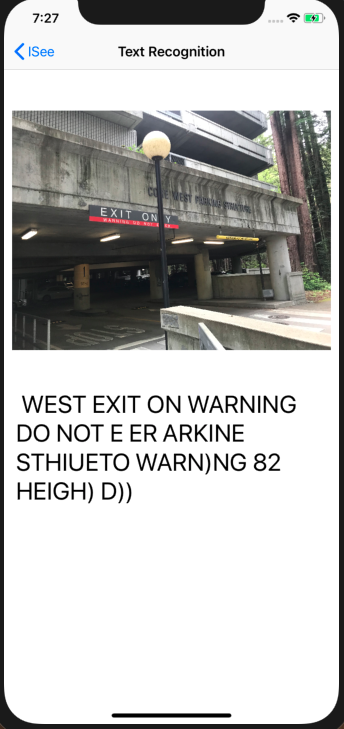
\includegraphics{Fig/parkingTextRecognition.png}}
  \hfill  
  \subfigure[Parking sign]{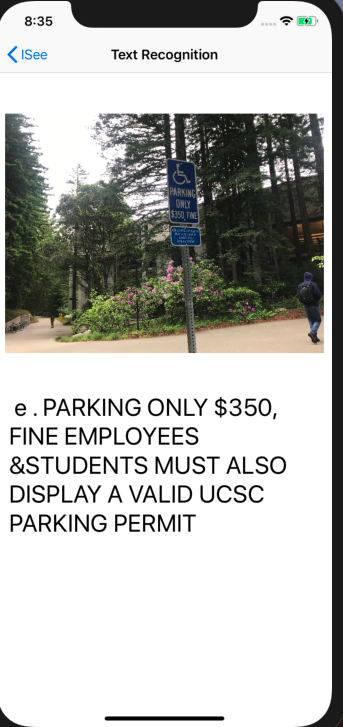
\includegraphics{Fig/parkingsignTextRecognition.png}}
  \hfill
\caption{Outdoor Image Text Recognition on IOS device}
\label{TextoutdoorIOS}
\end{figure}

The OCR API show some solid result for text recognition. For example, in Fig \ref{TextindoorIOS} (e) Dancing Studio, the app recognized "Please close doors when", it's hard for a regular user to notice the text in the image. Fig \ref{TextoutdoorIOS} (f) Parking sign, gives the useful information in the image. However, The OCR API not robust enough for blind users. First, it will return misleading information. For example, As shown in Fig \ref{TextindoorIOS} (c) Comic, the API mistake "IF" for "T". Second, the API didn't check the spell of the word. It will recognize some no meaning words, such as "temolats" in Fig \ref{TextindoorIOS}(b)Presentation, "AEEDENT" in Fig \ref{TextoutdoorIOS} (b)Road and "E Er ARKINE" in Fig \ref{TextoutdoorIOS} (e)Parking lot.

\subsection{Image labeling}

In order to test ISee's Image Labeling feature on IOS device, the author uses 6 indoor images and 6 outdoor images as input, and the output is shown in Fig \ref{LabelingindoorIOS} and Fig \ref{LabelingoutdoorIOS}.
 
 The Image labeling API gives more useful information that the blind user may interest in. In Fig \ref{LabelingindoorIOS} and Fig \ref{LabelingoutdoorIOS}, the application can give partly correct information. Fig \ref{LabelingindoorIOS} (a) Desk, has "toy", (b) Presentation has"presentation, event, room, desk, class, computer" Fig \ref{LabelingoutdoorIOS} (a) Beach has "Beach, sky, sand, bird", and (c) signpost has "vehicle, plant, road, car, building,wheel". At the same time, the API makes some interesting mistakes. First, it adds something that didn't exist in the image, such as Fig \ref{LabelingindoorIOS} (b) Presentation, no musical instrument exists. (c) Comic "Bird"  and so on. This may give misinformation to the blind user. Second, the API missed some distinct entities in the image. For example, people in Fig \ref{LabelingoutdoorIOS} (a) Beach and (e) Dancing Studio. People are important for blinder users. However, face recognition is separated from image labeling API.

\begin{figure}
\centering
\SetFigLayout{3}{2}
  \subfigure[Desk]{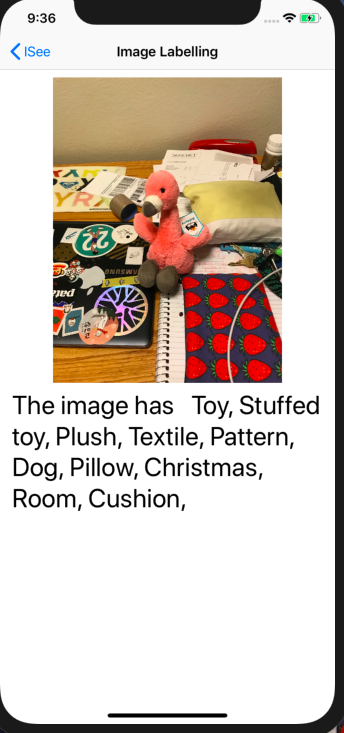
\includegraphics{Fig/FlamingoImageLabelling.png}}
  \hfill
  \subfigure[Presentation]{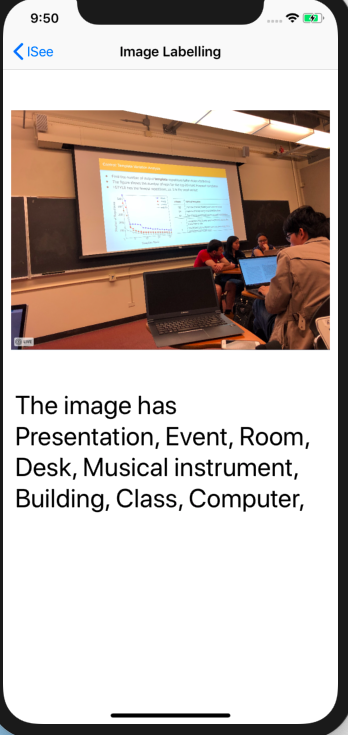
\includegraphics{Fig/ClassImageLabelling.png}}
  \hfill
  \subfigure[Comic]{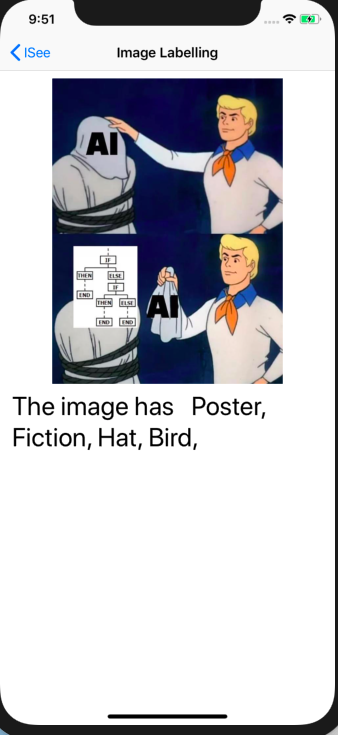
\includegraphics{Fig/AIImageLabelling.png}}
  \hfill
  \subfigure[Food]{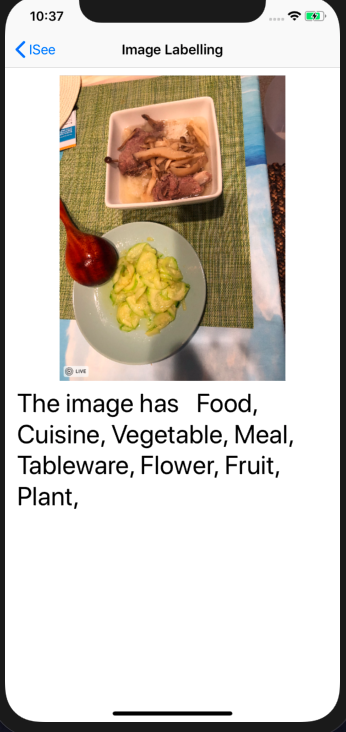
\includegraphics{Fig/foodImageLabelling.png}}
  \hfill
  \subfigure[Dancing Stuidio]{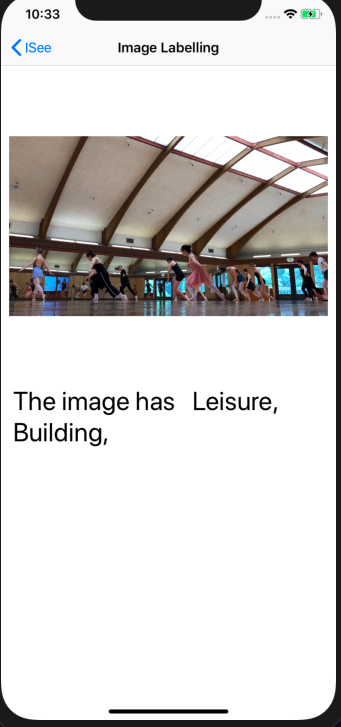
\includegraphics{Fig/BalletImageLabelling.png}}
  \hfill  
  \subfigure[
zebra crossing]{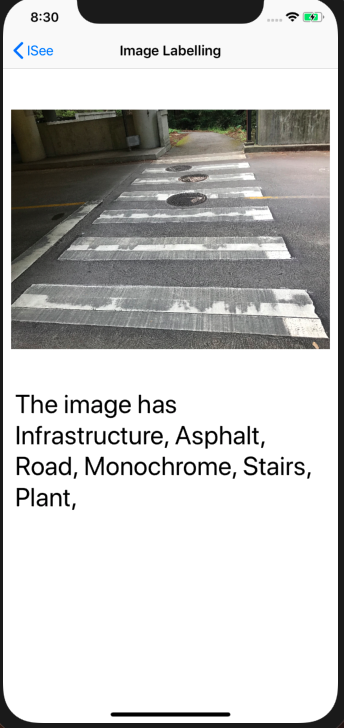
\includegraphics{Fig/RoadImageLabelling.png}}
  \hfill
\caption{Indoor Image Image Labeling on IOS device}
\label{LabelingindoorIOS}
\end{figure}

\begin{figure}
\centering
\SetFigLayout{3}{2}
  \subfigure[Beach]{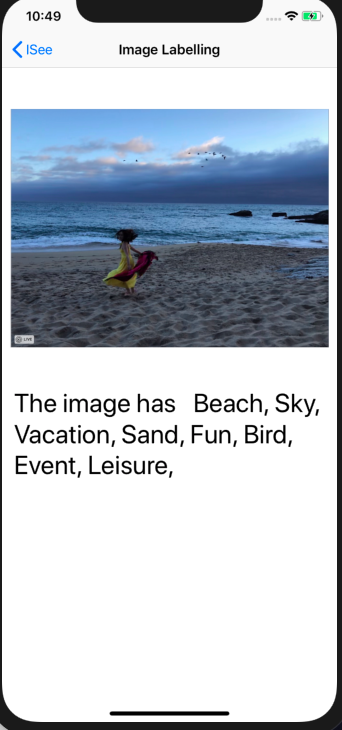
\includegraphics{Fig/BeachImgageLabelling.png}}
  \hfill
  \subfigure[Road]{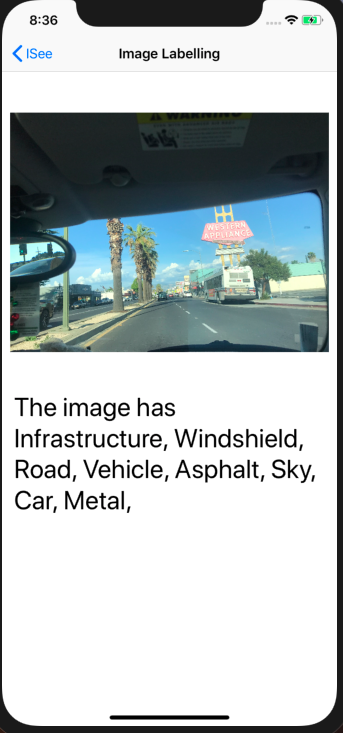
\includegraphics{Fig/carviewImageLabelling.png}}
  \hfill
  \subfigure[signpost]{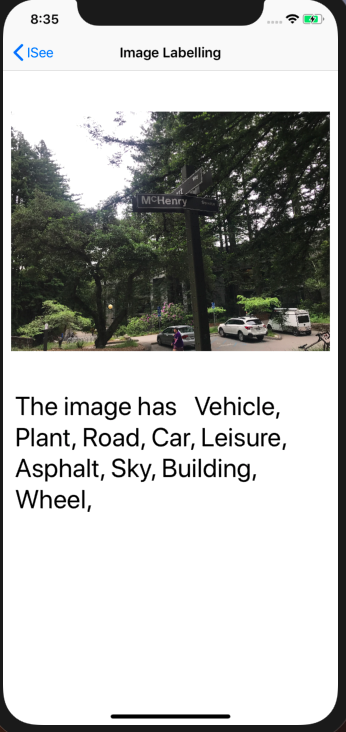
\includegraphics{Fig/signImageLabelling.png}}
  \hfill
  \subfigure[Library sign]{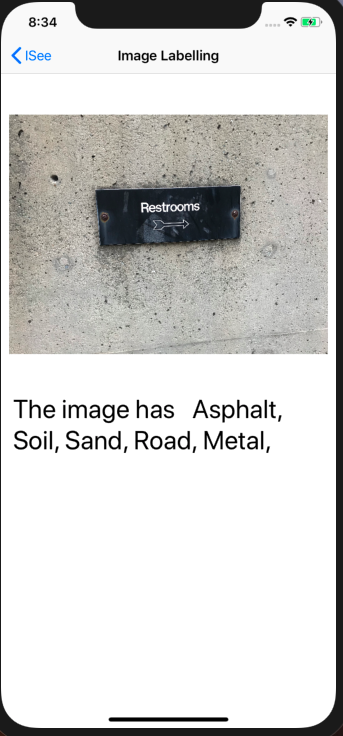
\includegraphics{Fig/RestroomsImageLabelling.png}}
  \hfill
  \subfigure[Parking lot]{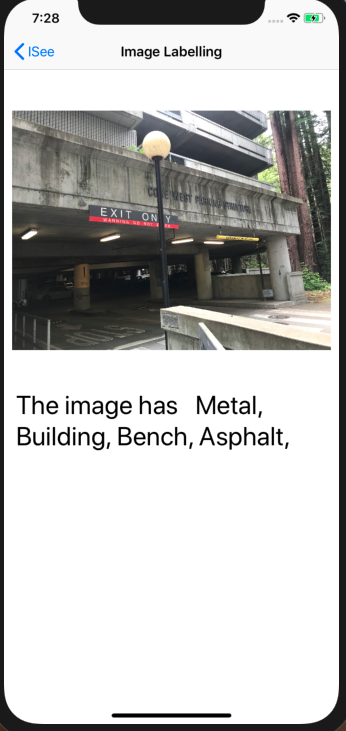
\includegraphics{Fig/parkingImageLabelling.png}}
  \hfill  
  \subfigure[Parking sign]{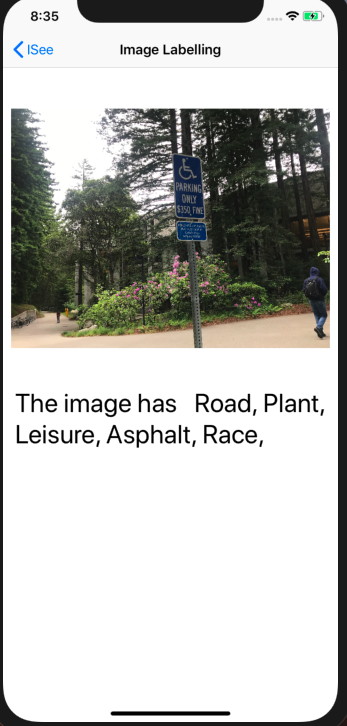
\includegraphics{Fig/parkingsignImageLabelling.png}}
  \hfill
\caption{Outdoor Image Image Labelling on IOS device}
\label{LabelingoutdoorIOS}
\end{figure}



\subsection{Text to Speech}
To test the text to speech feature on IOS device, the author uses the result from Optical character recognition or image labeling, add a template to the result.

For optical character recognition, if the text is detected, the template will be "the text in the image are + result Of OCR". Otherwise, the template will be "I am unable to detect any text in the image."

For image labeling, the template will be "The image has" + result from Image labeling +" in the image.

Test 6 images from Optical Character Recognition and 6 images from Image labeling. The template works fine, and the text to speech works fine.


\section{ISee on Android device}


\subsection{Optical Character Recognition}
The application is based on Firebase MLkit. 
In order to test ISee's optical character recognition feature on Android device, the author uses 6 indoor images and 6 outdoor images as input, and the output is shown in Fig \ref{TextoutdoorAndroid} and Fig \ref{TextoutdoorAndroid}.

\begin{figure}
\centering
\SetFigLayout{3}{2}
  \subfigure[Candy letters]{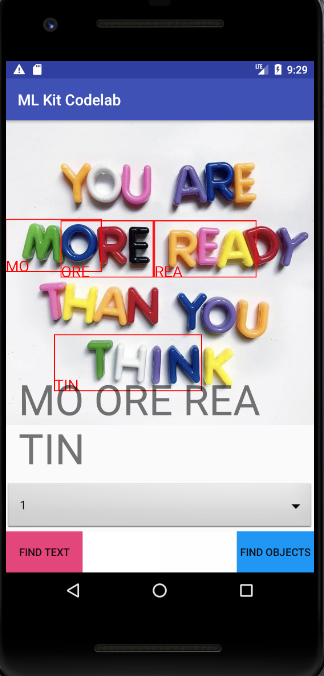
\includegraphics{Fig/androidyouareText.png}}
  \hfill
  \subfigure[SEM image]{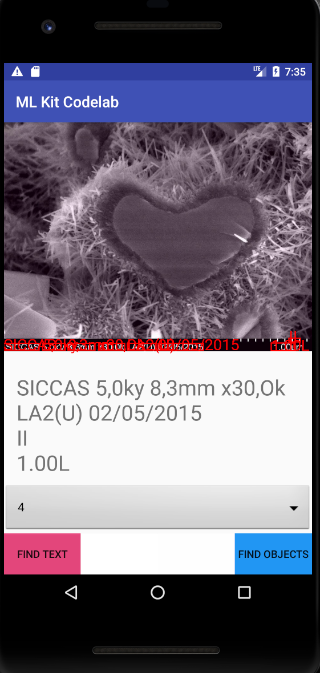
\includegraphics{Fig/andtext2.png}}
  \hfill
  \subfigure[NBA Oracle Arena]{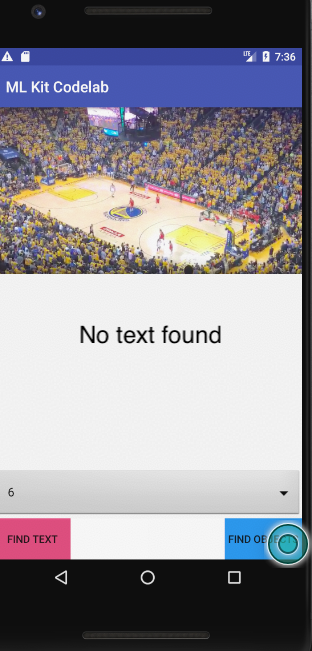
\includegraphics{Fig/androidplaytext1.png}}
  \hfill
  \subfigure[Handwriting]{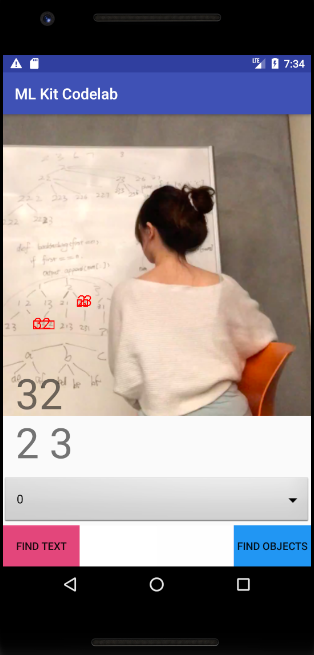
\includegraphics{Fig/andindoortext1.png}}
  \hfill
  \subfigure[slides]{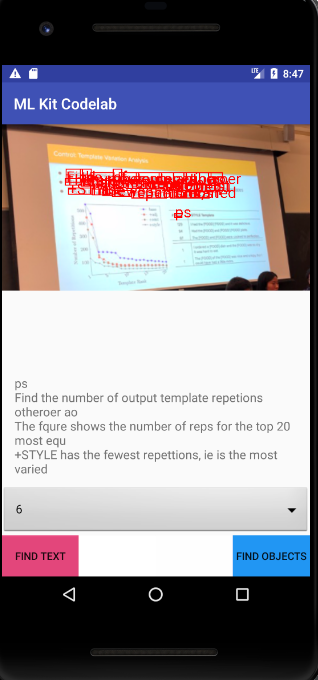
\includegraphics{Fig/andslidestext.png}}
  \hfill  
  \subfigure[Super market]{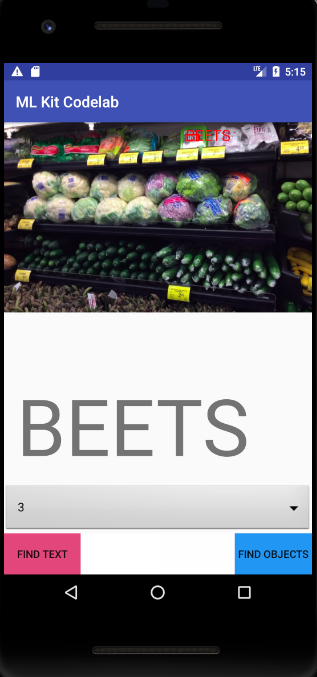
\includegraphics{Fig/andvegT.png}}
  \hfill
\caption{Indoor Image Text Recognition on Android device}
\label{TextindoorAndroid}
\end{figure}

\begin{figure}
\centering
\SetFigLayout{3}{2}
  \subfigure[Reno sign]{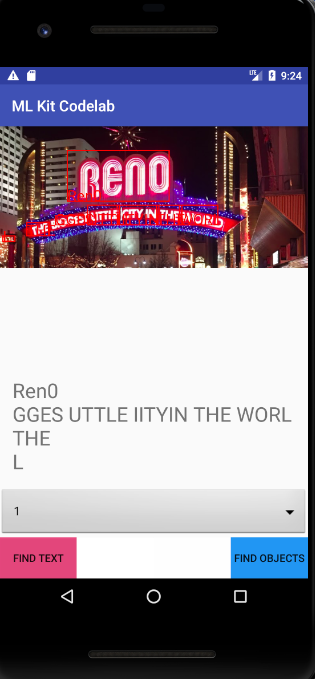
\includegraphics{Fig/androidrenotext.png}}
  \hfill
  \subfigure[Carpools sign]{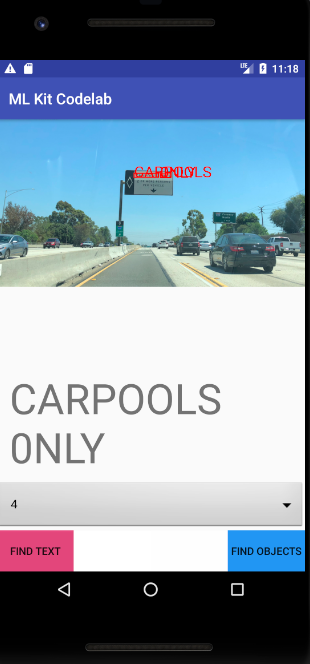
\includegraphics{Fig/an2.png}}
  \hfill
  \subfigure[Farm]{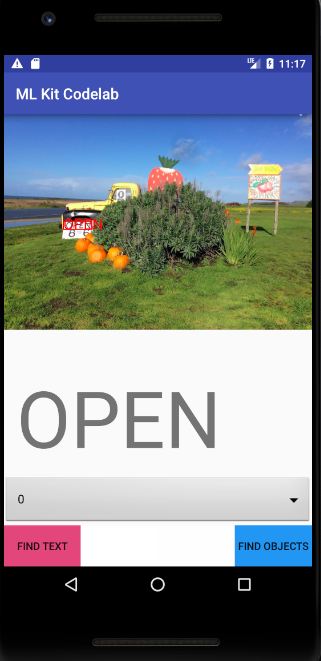
\includegraphics{Fig/an3.png}}
  \hfill
  \subfigure[UCSC sign]{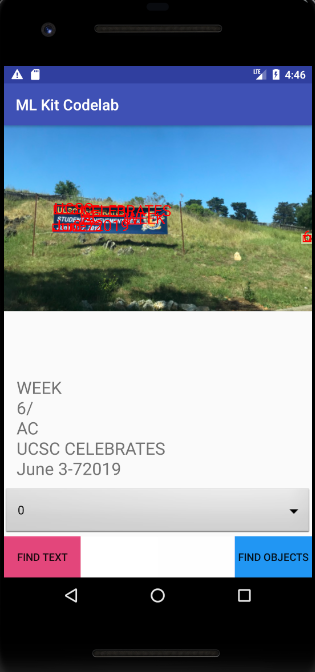
\includegraphics{Fig/anducsct.png}}
  \hfill
  \subfigure[License plate]{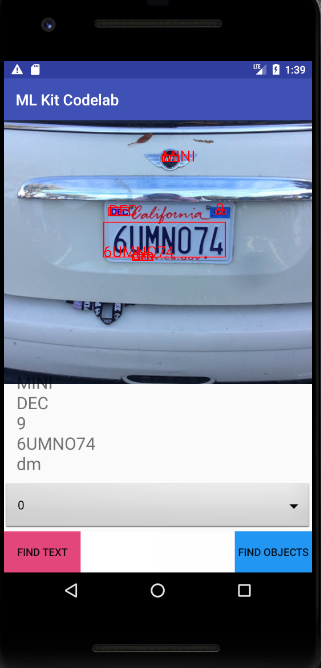
\includegraphics{Fig/an5.png}}
  \hfill  
  \subfigure[Building]{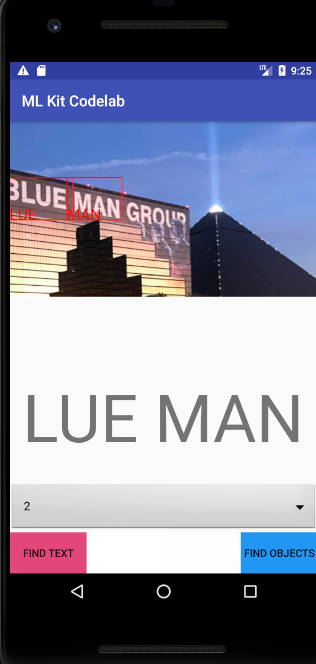
\includegraphics{Fig/androidBluetext.png}}
  \hfill
\caption{Outdoor Image Text Recognition on Android device}
\label{TextoutdoorAndroid}
\end{figure}

The Text recognition API show some amazing result in Fig \ref{TextoutdoorAndroid} (b)Carpools sign, (c) Farm and (e) License plate. It gives important and correct information in the image. However, the text recognition API didn't work well on handwriting Fig \ref{TextindoorAndroid} (d) and curled words \ref{TextoutdoorAndroid} (a). And couldn't recognize blur text in Fig \ref{TextindoorAndroid} (c).


\subsection{Image labeling}

 In order to test ISee's optical character recognition feature on Android device, the author uses 6 indoor images and 6 outdoor images as input, and the output is shown in Fig \ref{ImageindoorAndroid} and Fig \ref{ImageoutdoorAndroid}.
 
 The image labeling API gives more useful information of the image. Such as "crowd, event, Team, Sports" in Fig \ref{ImageindoorAndroid} (c) NBA Oracle Arena. "Presentation, event" in Fig \ref{ImageindoorAndroid} (e) Slides , "Food, vegetable" in Fig \ref{ImageindoorAndroid} (f)Super market, "Beach, sky ,cliff, Bird" in Fig\ref{ImageoutdoorAndroid}(a) Beach, "Sky, Field,vegetable, Farm, Road" in Fig\ref{ImageoutdoorAndroid} Farm, "Sky, sunset, vehicle, car" in Fig\ref{ImageoutdoorAndroid} (c) Sunset and so on.
The API also gives misinformation such as no "wheel, tire" in Fig\ref{ImageoutdoorAndroid} (e)License plate and no "dogk eyelash" in Fig \ref{ImageindoorAndroid} (e) Slides. 

\begin{figure}
\centering
\SetFigLayout{3}{2}
  \subfigure[candy letters]{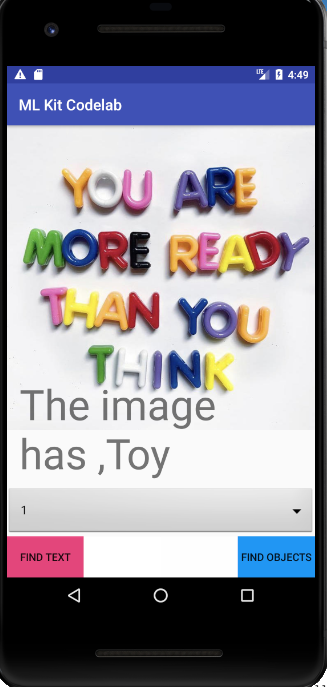
\includegraphics{Fig/andletteri.png}}
  \hfill
  \subfigure[SEM image]{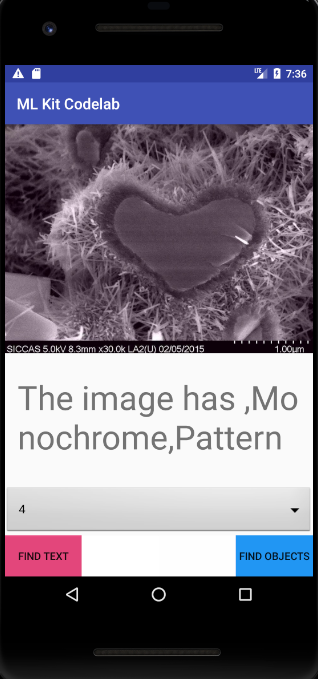
\includegraphics{Fig/andimage2.png}}
  \hfill
  \subfigure[NBA Oracle Arena]{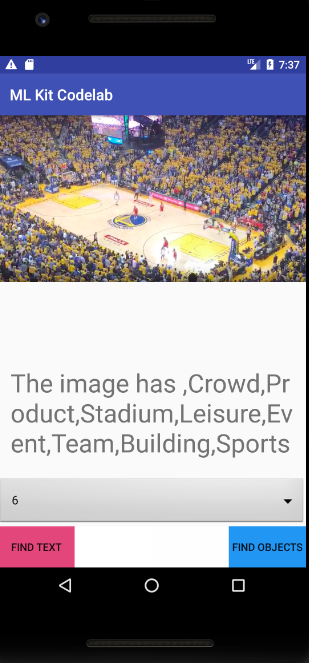
\includegraphics{Fig/androidplayimage.png}}
  \hfill
  \subfigure[Handwriting]{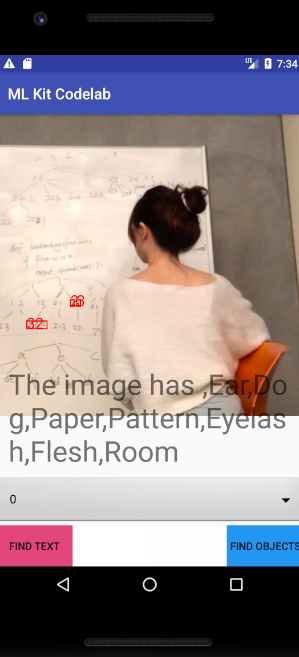
\includegraphics{Fig/andmeimagelable.png}}
  \hfill
  \subfigure[Slides]{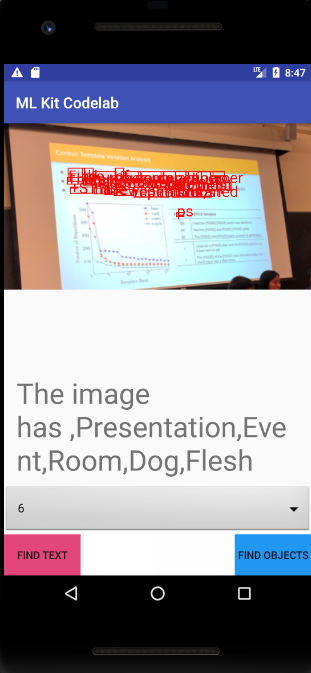
\includegraphics{Fig/andslidesimage.png}}
  \hfill  
  \subfigure[Super market]{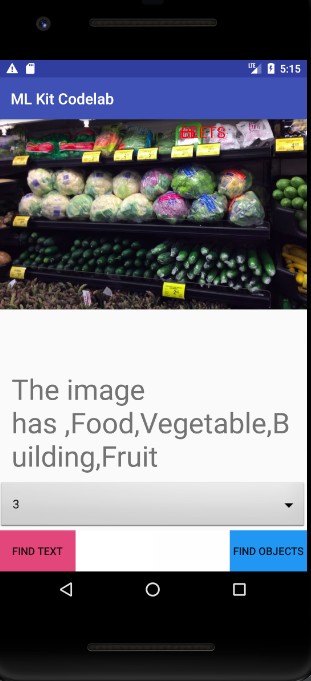
\includegraphics{Fig/andvegI.png}}
  \hfill
\caption{Indoor Image Image Labelling on Android device}
\label{ImageindoorAndroid}
\end{figure}



\begin{figure}
\centering
\SetFigLayout{3}{2}
  \subfigure[Beach]{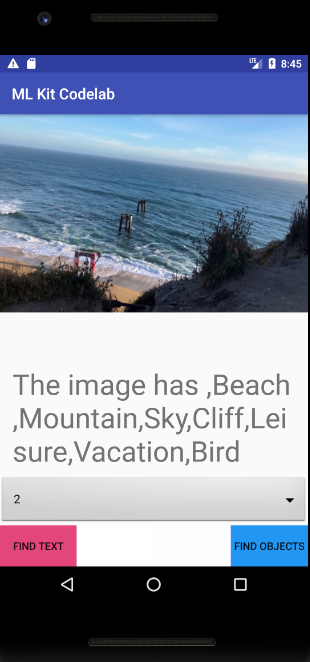
\includegraphics{Fig/androidseaImage.png}}
  \hfill
  \subfigure[Farm]{\includegraphics{Fig/andopeni.png}}
  \hfill
  \subfigure[Sunset]{\includegraphics{Fig/androidsunset.png}}
  \hfill
  \subfigure[UCSC sign]{\includegraphics{Fig/anducsci.png}}
  \hfill
  \subfigure[License plate]{\includegraphics{Fig/andcari.png}}
  \hfill  
  \subfigure[Beach]{\includegraphics{Fig/andSealI.png}}
  \hfill
\caption{Outdoor Image Image Labelling on Android device}
\label{ImageoutdoorAndroid}
\end{figure}



\subsection{Text to Speech}
To test the text to speech feature on Android device, the author uses the result from Optical character recognition or image labeling, add a template to the result.

For optical character recognition, if the text is detected, the template will be "the text in the image are + result of OCR". Otherwise, the template will be "I am unable to detect any text in the image."

For image labeling, the template will be "The image has" + result from Image labeling +" in the image.

Test 6 images from Optical Character Recognition and 6 images from Image labeling. The template works fine, and the text to speech works fine.


\section{MLkit OCR vs Blur Text Spotter}
In order to evaluate the performance of the blur text recognition Algorithm developed by Siyang Qin with ML kit, the author computes the false positive rate and truth positive rate of each of them.
\subsection{Data}
There are 939 images, as shown in Fig \ref{testimage}, labeled with ground truth. In the ground truth data, if an image is labeled as 'Skip,' it does not contain text. Otherwise, it contains text.
  \begin{figure}
    \centering
    \includegraphics[width =0.8\linewidth]{Fig/TestData.png}
    \caption{Test image }
    \label{testimage}
\end{figure}
 
 
 The heat map Images generated by Blur text Spotter are shown in Fig
\ref{Blurdata}. The white pixels in heat map images mean siyang's algorithm spots text. The black pixels in heat map images means no text spotted by siyang's algorithm. There are 552 heat map images with ground truth.


 \begin{figure}
    \centering
    \includegraphics[width =0.8\linewidth]{Fig/BlurData.png}
    \caption{The heat map images of Blur text Spotter}
    \label{Blurdata}
\end{figure}
 
 
\subsection{Experiment}
The code for the experiment can be found:https://github.com/WaitingZhan/MLkit-vs-Siyang
\subsubsection{MLkit experiment}
The author uses MLKit API processed 939 images with ground truth and generated the result of MLKit. In the result of MLkit, '0' means no text found by MLKit API for that image; otherwise, the connect is the text found by MLKit API.
 
For each image, a False Positive is defined as when MLKit finds text and the ground truth label is 'Skip'. A True Positive is defined when MLKit finds text and the label is not 'Skip'.

True Positive Rate(TPR) is defined as:
\begin{equation*}
    True Positive Rate =\frac{The number of True Positive in the dataset}{The size of the dataset}
\end{equation*}

False Positive Rate(TPR) is defined as:
\begin{equation*}
    False Positive Rate =\frac{The number of False Positive in the dataset}{The size of the dataset}
\end{equation*}

\subsubsection{Siyang's algorithm experiment }
For siyang's algorithm, the text were found when the number of largest connected white pixels is greater than the number of N. The range of N is defined by the range of the number of largest connected white pixels.

For each heat map image, a False Positive is defined as when siyang's algorithm finds text and the ground truth label is 'Skip'. A True Positive is defined as when siyang's algorithm finds text and the label is not 'Skip'.



In the range of N, the author calculate True Positive Rate(TPR) and Faulse Positive Rate(FPR) for each N, and then generated the Receiver Operating Characteristic (ROC) curve.



 
 \subsection{Result}
 \subsubsection{ML Kit OCR result}

 
The author tests 910 images with labeled ground truth on MLkit. There are 53 images when MLKit finds text and the ground truth label is 'Skip'. There are 843 images when MLKit finds text and the label is not 'Skip'.The false positive rate (FPR) for MLkit Text recognition is 0.057, and the true positive rate (TPR) for MLkit is 0.942. Here is some example from MLkit shown in Fig \ref{MLKitrTRR}. The MLkit is unable to detect the blurred image, only identify 1 out of 4 images with the number "204".
 
 
  \begin{figure}
    \centering
    \includegraphics[width =0.8\linewidth]{Fig/MLreult.png}
    \caption{ML kit text recognizer result}
    \label{MLKitrTRR}
\end{figure}
 
 
 
 \subsubsection{Blur Text Sport result}

552 images have a heat map and ground truth. Among these 552 images, only 1 image with ground truth "skip" has at least 1 connected white pixel (24 pixels). N is range from 1 to 162. The ROC curve is shown in Fig \ref{ROC}. 
   \begin{figure}
    \centering
    \includegraphics[width =0.8\linewidth]{Fig/ROC.png}
    \caption{Receiver Operating Characteristics for siyang's Algorithm}
    \label{ROC}
\end{figure}

\chapter{Conclusion}
The project made an ISee application for blinder user or visually impaired user on IOS device and Android device. ISee can read the text and the entity in the image for a blind user. The accuracy of the ISee depends on Google Firebase Text recognition API and Image Labeling. The performance of ISee is not enough for navigation, just offer a glimpse of the real world to a blind user. The author also computes the false positive rate and truth positive rate of MLkit's text recognition and blur text recognition Algorithm developed by Siyang Qing. Using 939 images with labeled ground truth, the FPR for MLkit is 0.057, and TPR for MLkit is 0.942.

 



\appendix
\chapter{Compiling}
The code for the project can be found:https://github.com/WaitingZhan/ISee.

The code for comparison between ML kit text recognizer and siyang's blur text algorithm can be found: https://github.com/WaitingZhan/MLkit-vs-Siyang.


Prerequisites for firebase:
\section{System Prerequisite for IOS}
\textbf{iOS 11.4}


\textbf{Xcode 10.1}


\textbf{Swift 4.2}


\textbf{Firebase}

\textbf{AVSpeechSynthesizer}


\section{System Prerequistie for Android}
\textbf{Android Studio Version 3.4.1} 


\textbf{Java SE 10}


\textbf{Firebase Targets API level 16 (Jelly Bean) or later
Uses Gradle 4.1 or later}

\textbf{Text to speech}

\section{MLkit Text recognition vs Siyang's Algorithm}
\textbf{Python 3.7.1}
\textbf{Jupyter notebook}


% %%%%%%%%%%%%%%%%%%%%%%%%%%%%%%%%%%%%%%%%%%%%%%%%%%%%%%%%%
% bibliography

% 2010june01 sol katzman:
% if \nocite is specified, all entries in the bib file are included,
% probably not what you want, so comment out the \nocite and only get the cited references.
%\nocite{*}

% 2010june01 sol katzman:
% this makes the bibliography single spaced, with double spacing between entries
\def\baselinestretch{1.0}\large\normalsize

\bibliographystyle{plain}
\bibliography{uctest}
\begin{acknowledgements}
The author, thanks to Professor Roberto Manduchi and for his feedback and helpful suggestions.

\\
The author thanks Hyein Jeong for the data collection in the project.

\\ The author thanks Suzanne da Camara, and Bill for grammar checking.

\\ The author thanks Professor J. J. Garcia-Luna-Aceves for reading the report.

\\The author thanks sifang you.

\end{acknowledgements}

\end{document}